\chapter{The Reconstruction Algorithm}

\section{Basis}

Our reconstruction uses the $\chi^2$ metric to determine which ordering of hits is best. Each triple represents one term in the sum of equation \ref{eq:chi2}. Since better orderings of hits produce more similar $\eta$ values, the ordering with the lowest value of $\chi^2$ is the most probable one. Therefore, we must try each possible ordering of hits in order to find the one that is best - a very computationally complex calculation. If there are $N$ hits in a photon event, there are $N!$ possible orderings of those hits, and we must recalculate the eta value for each hit in each ordering, adding an additional factor of $N$, to give us a total run-time of $O(N*N!)$ for each photon. There are several heuristic improvements we can make to this algorithm to shorten the average-case run-time, but we start with a basic iterative and sequential approach for simplicity's sake. The full pseudo-code for this approach is shown in Algorithm \ref{alg:seq}.

\begin{algorithm}
\caption{Sequential Reconstruction Algorithm}\label{alg:seq}
\begin{algorithmic}
\For {each photon}
    \State $n \gets$ \# hits for photon $i$
    \State min$\chi^2 \gets$ max double
    \State bestPermutation $\gets 0$
    \For {permutation $j \in$ all $n!$ permutations}
        \State $\chi^2 \gets 0$
        \For {hit $k\in 1...n-1$}
            \State // Calculate spatial angle:
            \State $\vec{x}_k \gets$ position of hit k
            \State $\hat{r}_k \gets |\vec{x}_{k+1} - \vec{x}_k|$ \Comment{Unit vector along photon direction}
            \State $\eta_k = \cos{\phi_k} = \hat{r}_k\cdot\hat{r}_{k-1}$ \Comment{From dot product equation}
            \State
            \State // Calculate energy angle:
            \State $W_k = \frac{1}{m_e c^2}\sum_{i=k+1}^n E_i$ \Comment{Unitless energy; energy before hit k}
            \State $\eta'_k = \cos{\phi'_k} = 1 + \frac{1}{W_{k-1}}-\frac{1}{W_k}$ \Comment{From Compton equation}
            \State
            \State // Calculate Errors:
            \State $\delta\eta_k^2 = \delta\phi_{k,r}^2\sin^2(\phi_k)$ \Comment{$\delta\phi_{k,r}$ depends on $\delta x,\delta y,\delta z$}
            \State $\delta\eta'^2_k = \frac{\delta W_{k-1}^2}{W_{k-1}^4}+\delta W_k^2 \big[(\frac{1}{W_k^2}-\frac{1}{W_{k-1}^2})^2 - \frac{1}{W_{k-1}^4}\big]$
            \State
            \State // Add to $\chi^2$:
            \State $\chi^2 \gets \chi^2 + \frac{1}{n-2} \frac{(\eta_k-\eta'_k)^2}{\delta\eta_k^2 + \delta\eta'^2_k}$
        \EndFor
        \State
        \If{$\chi^2 <$ min$\chi^2$}
        \State min$\chi^2 \gets \chi^2$
        \State bestPermutation $\gets j$
        \EndIf
    \EndFor
    \State
    \State // Predict $\eta$:
    \State $\eta_{pred} = 1 + \frac{1}{W_0}-\frac{1}{W_1} \pm \delta\eta'_1$
    \State
\EndFor
\end{algorithmic}
\end{algorithm}

\section{Performance improvement}
Though it is difficult to improve the worst-case time complexity of our algorithm, it is possible to make several changes that decrease the average run-time per photon. The most important of these changes is the switch from an iterative approach to a tree search, and the use of parallelism.

\subsection{Tree search}
The first and perhaps most important performance improvement we make is to change the structure of our program from an iterative approach - testing each sequence individually, one after another - to a recursive tree search, shown in Algorithms \ref{alg:recon} and \ref{alg:recurse}. Each photon has its own tree, which refers to a type of data structure in computer science, containing 'nodes' of information - in our case, possible paths of the photon. Each parent node has a series of child nodes (excluding those at the end of the sequence), and to search the tree we simply have to choose a path through it, keeping track of the $\chi^2$ value as we go. Once we have searched each path we consider possible, we assume the path with the lowest $\chi^2$ value is the correct one and return its first two hits.  The first two hits are then all we need to estimate the scattering angle of the initial photon. This is an improvement on our sequential algorithm, as we do not have to re-compute $\chi^2$ for each node with the same parent sequence, instead simply adding onto it each time we process a new node.

In our program, the nodes of our search tree each contain a Hit (a location and energy deposit) and a $\chi^2$ value for that point in the sequence. As we cannot start calculating the $\chi^2$ value without at least one triple, we first take each possible pair of hits and run them through our recursive search algorithm (line \ref{ln:combo}, algorithm \ref{alg:recon}), keeping a running tally of the $\chi^2$ value and updating it for each child node we process (line \ref{ln:chi2}, algorithm \ref{alg:recurse}). Theoretically, we would still have to process every possible sequence before reaching a conclusion about the minimum $\chi^2$ value, but, as discussed in the following sections, there are other ways to decrease the average-case runtime. The real performance improvement of the tree comes from the recursive approach. In our iterative approach, we recalculated $\chi^2$ for each node, including those which had the same parent node (giving them the same $\chi^2$ value). In the recursive approach, we cut down on these repeat calculations by carrying the $\chi^2$ value through each sequence and only adding onto it when we process a new node. 

\begin{algorithm}
\caption{Main tree search reconstruction algorithm}\label{alg:recon}
\begin{algorithmic}[1]
\State \#pragma omp parallel \Comment{Run each photon in parallel} \label{ln:parallel}
\For {each photon}
    \State $n \gets$ \# hits for photon $i$
    \State
    \For {each triple} \label{ln:precompute} \Comment{Precompute spatial angles, $\eta_i$}
        \State triples[i][j][k] = $\hat{r}_j\cdot\hat{r}_k$ \Comment{Hit $j$ is the vertex}
    \EndFor
    \State
    \State min$\chi^2 \gets$ max\_value \Comment{Initialize min values}
    \State firstTwoHits $\gets$ NULL
    \State
    \For {each combination of hits 0 and 1} \label{ln:combo}
        \State $\chi^2 \gets$ findOptRecursive(hit 0, hit 1, $n$, 0) \Comment{Test each pair of hits}
        \State
        \If{$\chi^2 <$ min$\chi^2$} \Comment{Check for most likely permutation}
        \State min$\chi^2 \gets \chi^2$
        \State firstTwoHits $\gets$ hits 0 and 1 \Comment{Reset first two hits}
        \EndIf
    \EndFor
    \State
    \State $\eta'_0 = 1 + \frac{1}{W_0}-\frac{1}{W_1} \pm \delta\eta'_0$ \Comment{Predict $\eta'$ from first two hits}
    \State
\EndFor
\end{algorithmic}
\end{algorithm}

\begin{algorithm}
\caption{Recursive function in tree search}\label{alg:recurse}
\begin{algorithmic}[1]
\Function{findOptRecursive}{hit 0, hit 1, $n$, $\chi^2$}
    \State n\_left = n - hitsUsed \Comment{Set recursion depth}
    \If{n == n\_left}  \Comment{Base case}
        \State \Return $\chi^2$
    \EndIf
    \State
    \For{hit 2 = each possible next hit}
        \State Calculate the new energy angle:
        \State $W \gets W - \frac{1}{m_e c^2}E_2$ \Comment{Calculate change in energy}
        \State $\delta W^2 \gets \delta W^2 - \frac{1}{m_e c^2}\delta E_2^2$
        \State
        \State Calculate $\eta'$ and $\delta \eta'$ \Comment{See algorithm \ref{alg:seq}}
        \State $\eta \gets$ triples[0][1][2] \Comment{$\delta\eta$ is constant}
        \State
        \State Calculate new$\chi^2$ from $\eta, \eta', \delta\eta, \delta\eta'$ \Comment{See algorithm \ref{alg:seq}} \label{ln:chi2}
        \State
        \If{new$\chi^2 > \chi^2$[p-value]} \Comment{Prune with $\chi^2$ lookup table} \label{ln:pval}
            \State \textbf{continue}
        \EndIf
        \State
        \State findOptRecursive(hit 1, hit 2, $n-1$, new $\chi^2$) \Comment{Move on to next hits}
    \EndFor
\EndFunction
\end{algorithmic}
\end{algorithm}

\subsection{Pre-calculation of $\eta$ values}
Another performance improvement comes from pre-calculating the spatial angles for each triple, shown in algorithm \ref{alg:recon} line \ref{ln:precompute}. In the sequential/iterative algorithm, we calculate $\eta$ for each triple in each sequence, but unlike $\eta'$, the spatial angle does not change based on the previous ordering of hits. As it is only based on the hits in its given triple, we can calculate $\eta$ once for each possible triple before we start the tree search and fetch the values when they come up in order to reduce our run-time per photon.

\subsection{$\chi^2$ and $\eta$ cutoffs}

During our tree search, we can 'prune' some sub-trees by filtering out some possible sequences before we reach the final recursion depth. Theoretically, we could still end up having to search the whole tree for the correct path depending on the input ordering of the hits, but generally these methods will improve our runtime in the average case. We prune a sub-tree if:
\begin{enumerate}
    \item The $\chi^2$ value is already greater than the running minimum.
    \item The energetically reconstructed cos(angle), $\eta'$, is greater than 1 by some amount.
    \item The $\chi^2$ value exceeds what we would expect for a given p-value.
\end{enumerate}
The p-value of an ordering is related to the probability of getting some $\chi^2$ value with the number of degrees of freedom as the number of hits we have added to the value so far. We use a look-up table to find the estimated $\chi^2$ value, such as the one shown in figure \ref{fig:p-val}, and compare it to our current $\chi^2$ value (algorithm \ref{alg:recurse} line \ref{ln:pval}). For example, if we choose a p-value of 0.10, we will not accept any orderings that have less than a 10\% chance of being correct. So, from the table, we will cut off computation for $\chi^2$ values greater than 2.76 for one hit, 4.605 for two hits, 6.251 for three hits, etc.

\begin{figure}
    \centering
    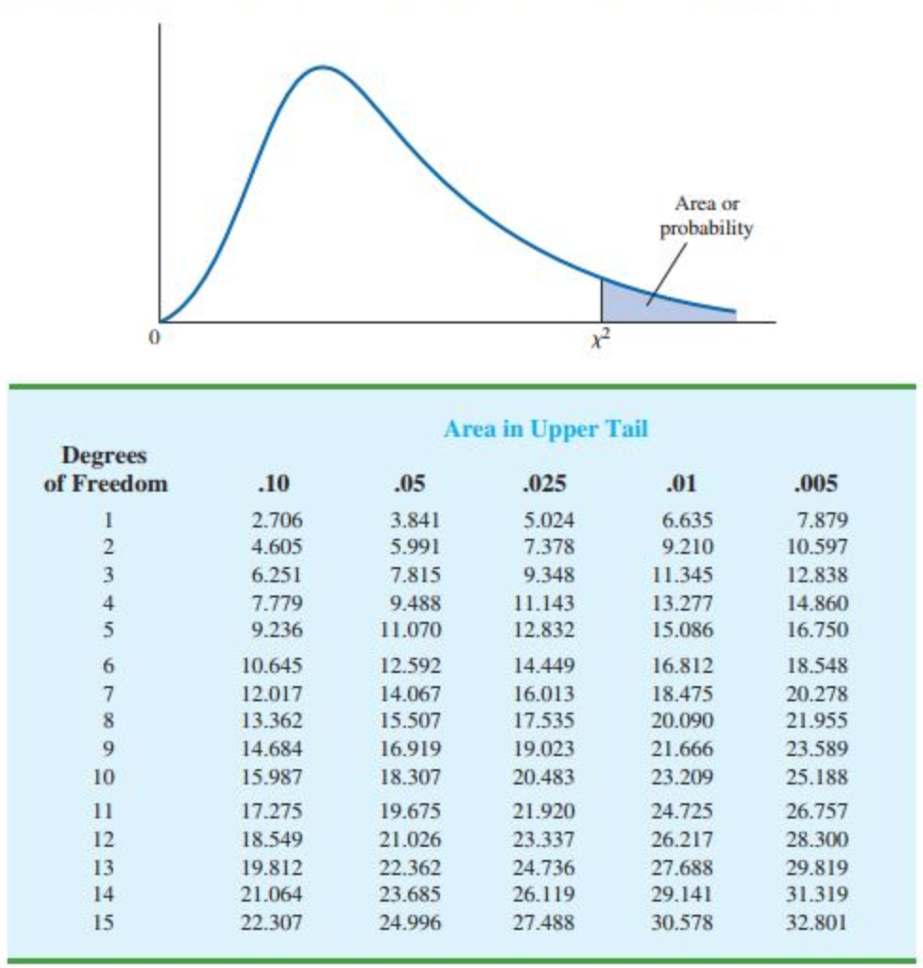
\includegraphics[width=0.5\textwidth]{chi2table.png}
    \caption{An example $\chi^2$ look-up table \cite{chitable}.}
    \label{fig:p-val}
\end{figure}

\section{Parallelism}
Our final performance improvement comes from parallelism - each photon's computation may be run in parallel with the others' to reduce the total running time of our algorithm (algorithm \ref{alg:recon} line \ref{ln:parallel}). This means that if any given photon's computation takes longer than real-time there will not be a backlog of events to process, which would delay the localization of a gamma-ray burst or other transient. The easier photons to process, with fewer numbers of hits, will naturally complete first. This is perfect for our problem, as we expect there to be more photons with small numbers of hits than those with larger numbers of hits. If we need a quick reading of a GRB source, we can get a broader position first using these easier-to-calculate photons and allow the more complicated events to increase the accuracy of our estimate after the fact.

As our current level of parallelism was able to adequately meet our time constraints, we do not run any other part of our computation in parallel, but there are several different ways we could implement this depending on future time constraints. For longer computations, we could save time by running a certain number of sub-trees in parallel threads and finding the lowest $\chi^2$ afterward. We could also calculate some of the spatial angles in parallel, as these have $N^3$ time complexity.

\section{Comparison}

The improvements we made to our algorithm made a significant difference in terms of overall performance. The sequential/iterative version of the algorithm could process only about 1000 photons per second, while the tree search algorithm can process over 50,000/sec at its best performance.